\normaltrue \difficilefalse \tdifficilefalse
\correctiontrue

%\UPSTIidClasse{11} % 11 sup, 12 spé
%\newcommand{\UPSTIidClasse}{11}

\exer{Diagramme de Bode$\star$ \label{C2:02:510_03}}
\setcounter{question}{0}\marginnote{\xpComp{SLCI}{11}}%\UPSTIcompetence[2]{C2-02}
\index{Compétence C2-02}\index{Compétence SLCI-11}
\index{Diagramme de Bode}
\ifcorrection
\else
\marginnote{\textbf{Pas de corrigé pour cet exercice.}}
\fi




\question{Tracer le diagramme de Bode de la fonction de transfert suivante : $F_3(p)=\dfrac{40}{p\left(1+300p\right)}$.}
\ifprof

\textbf{Tracer asymptotique}

\begin{marginfigure}
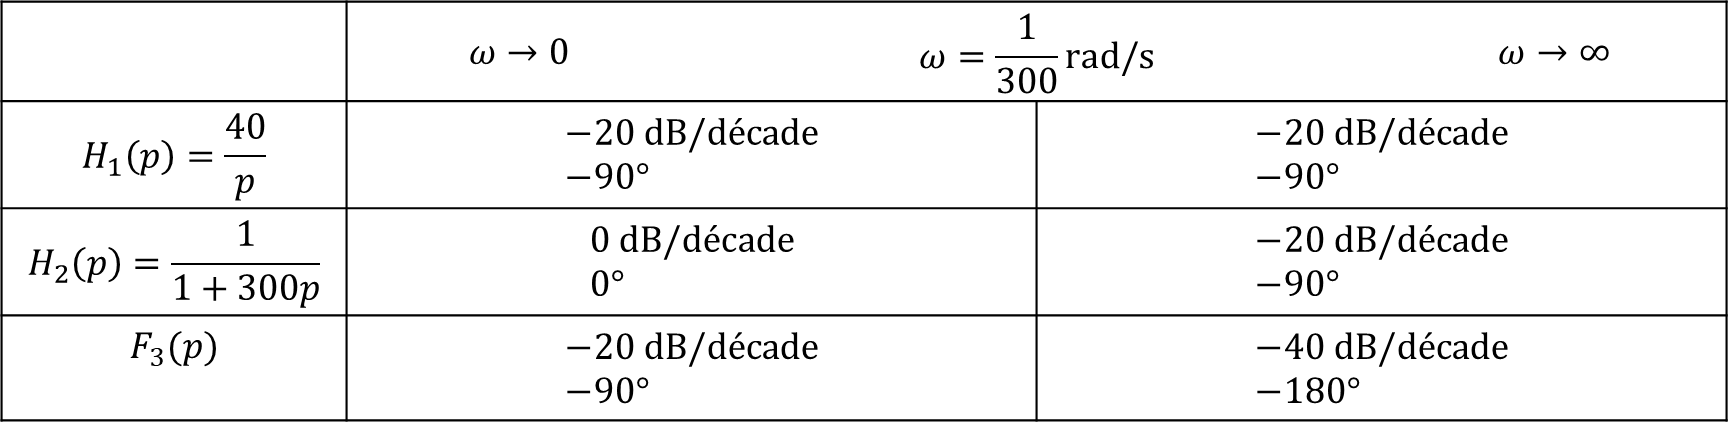
\includegraphics[width=\linewidth]{tab_03}
\end{marginfigure}


\textbf{Positionnement du diagramme de gain}
Lorsque que $\omega$ tend vers 0, $F_3(p)\simeq \dfrac{40}{p}$. Cette asymptote de pente \SI{-20}{dB/decade} passe par le point $(40,0)$. 


\begin{figure}[!h]
 \begin{tikzpicture}[xscale=2]
\tikzset{
semilog lines/.style={thin, bleuxp}, 
semilog lines 2/.style={semilog lines,bleuxpc},
semilog half lines/.style={semilog lines 2,dotted },
semilog label x/.style={semilog lines,below,font=\tiny,black},
semilog label y/.style={semilog lines,right,font=\tiny,black}
}
\begin{scope}[yscale=1/60]
\semilog{-4}{-1}{-40}{120}

\BodeAmp[orangexp,thick]{-4:-1}{\POAmpAsymp{40.}{300.}+\IntAmp{1}}
\BodeAmp[orangexp,ultra thick]{-4:-1}{\POAmp{40}{300}+\IntAmp{1}}
%\draw (-2.2,27) node {\footnotesize 23,5 dB, 0 dB/d\'ecade};
\draw (-3.5,120) node {\footnotesize $-$20 dB/d\'ecade};
\draw (-1.5,65) node {\footnotesize $-$40 dB/d\'ecade};
\draw [dashed,ultra thick,bleuxp] (-2.47,-1) -- (-2.47,80);
\draw (-2.47,-1)  node {\Huge $\cdot$} node [above right]{\footnotesize $\dfrac{1}{300}$};
\end{scope}
\begin{scope}[yshift=-2cm,yscale=1/90]
\UniteDegre
\OrdBode{45}
\semilog{-4}{-1}{-180}{0}
\BodeArg[orangexp,samples=200,thick]{-4:-1}{\POArgAsymp{40.}{300.}+\IntArg{1}}
\BodeArg[orangexp,ultra thick]{-4:-1}{\POArg{40}{300}+\IntArg{1}}
\end{scope}
\end{tikzpicture}
\end{figure}

%\begin{marginfigure}
%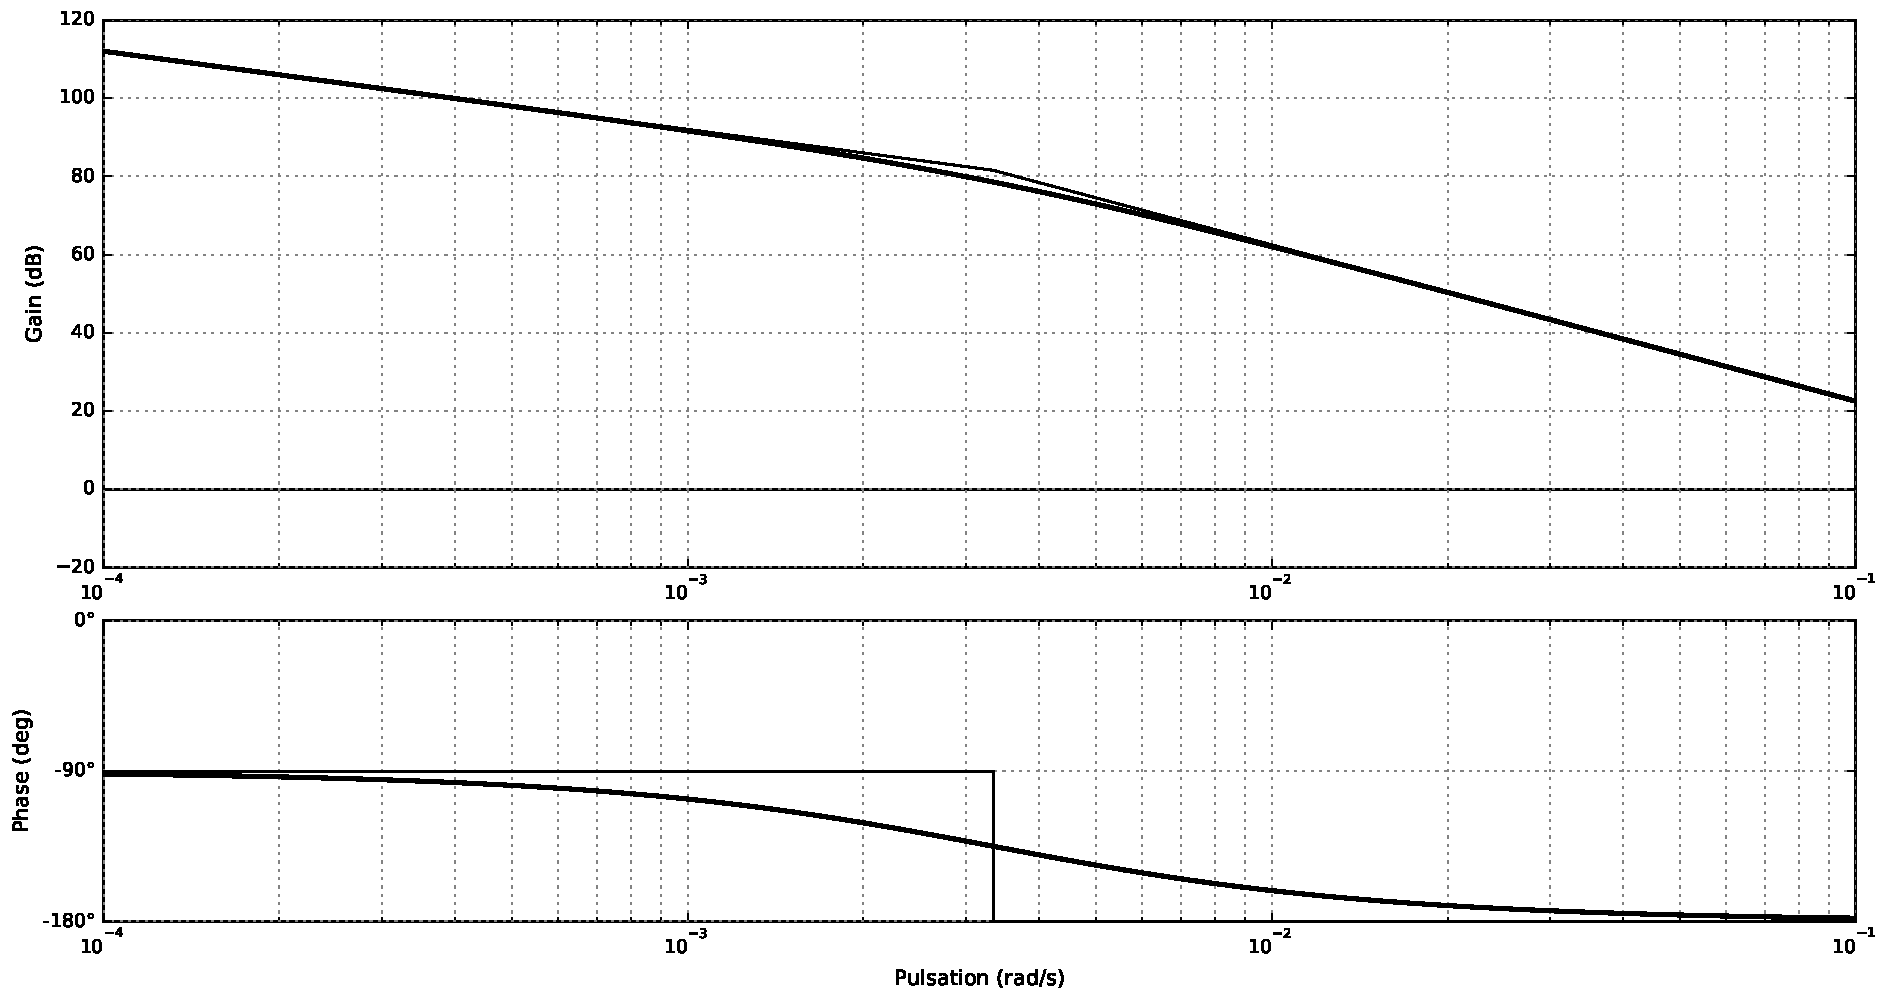
\includegraphics[width=\linewidth]{bode_03}
%\end{marginfigure}

\else 


\begin{figure}[!h]
 \begin{tikzpicture}[xscale=3]
\tikzset{
semilog lines/.style={thin, bleuxp}, 
semilog lines 2/.style={semilog lines,bleuxpc},
semilog half lines/.style={semilog lines 2,dotted },
semilog label x/.style={semilog lines,below,font=\tiny,black},
semilog label y/.style={semilog lines,right,font=\tiny,black}
}
\begin{scope}[yscale=1/60]
\OrdBode{20}
\semilog{-4}{-1}{-40}{120}

\end{scope}
\begin{scope}[yshift=-2cm,yscale=1/90]
\UniteDegre
\OrdBode{45}
\semilog{-4}{-1}{-180}{90}
\end{scope}
\end{tikzpicture}
\end{figure}

%\begin{marginfigure}
%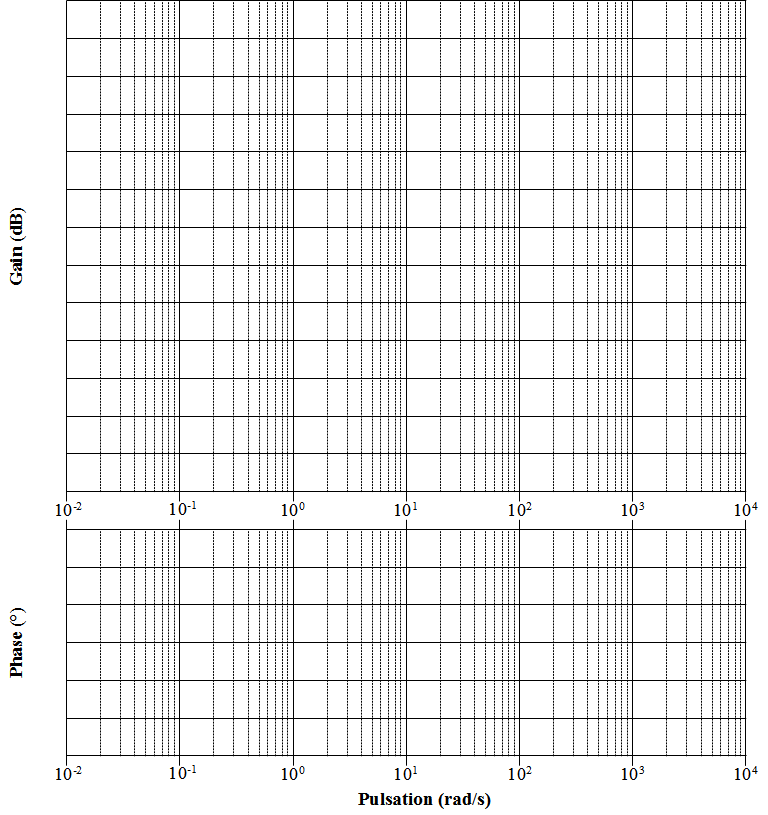
\includegraphics[width=\linewidth]{510_01}
%\end{marginfigure}
\fi





%\question{Réaliser le schéma-blocs.}
%\ifprof
%\begin{figure}[H]
%\centering
%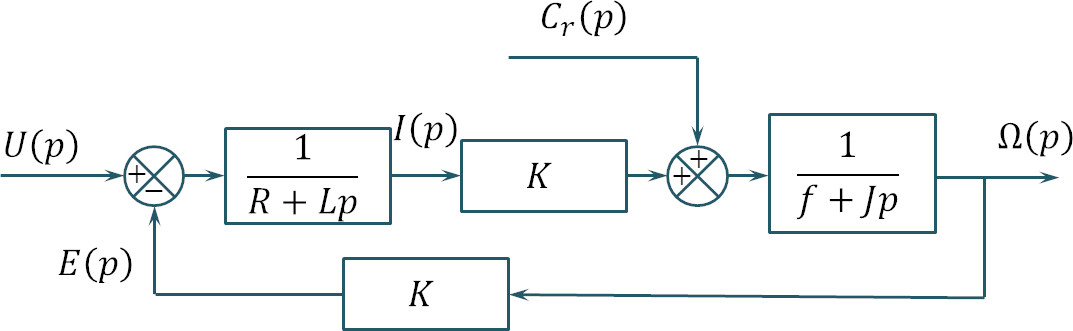
\includegraphics[width=\linewidth]{51_01_c}
%%\caption{Évolution du couple utile en fonction de la vitesse de rotation pour des
%%fréquences de commande de \SI{90}{Hz} à \SI{110}{Hz}. \label{fig_50_04}}
%\end{figure}
%\else
%\fi



\ifprof
\else

\marginnote{Corrigé voir \ref{C2:02:510_03}.}

\fi